\section{Experimento 3}

El último experimento presentado fue realizado en una oficina con aproximadamente 20 empleados trabajando, en horario laboral. La captura de paquetes se realizó sobre la red wifi de la empresa a la que se conectan la mayoría de los dispositivos móviles y notebooks.

\subsection{Resultados}

Para la primera fuente,  esperaremos que la informacíon del símbolo que representa a los paquetes broadcast sea mayor, debido a que la comunicación entre dispositivos tiende a ser unicast y no broadcast por lo que la cantidad de unicast es mayor.

\begin{figure}[H]
  \centering
  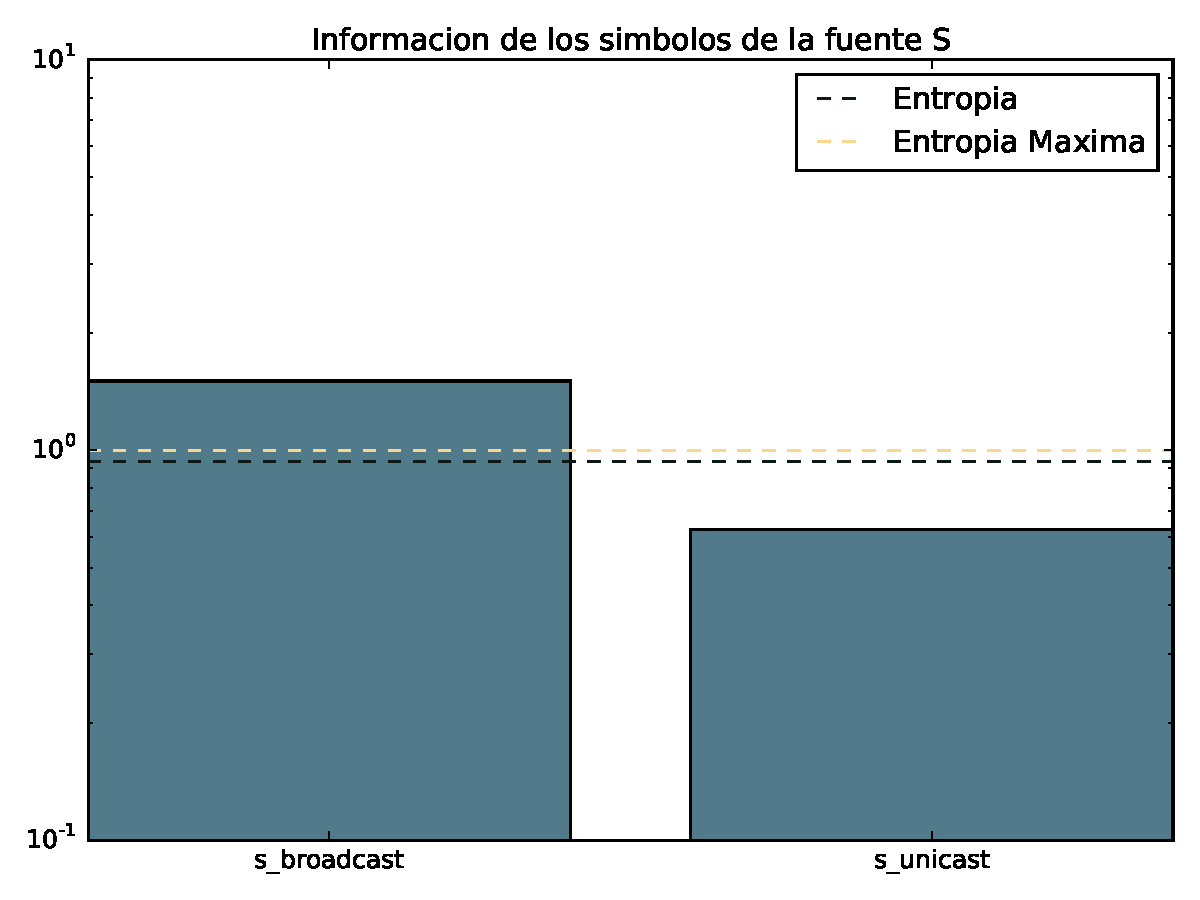
\includegraphics[width=8.5cm]{exp_empresa/grafico1.pdf}
  \caption{\normalfont }
\end{figure}

Esta red, al igual que la red analizada en el primer experimento corresponde a una red inalámbrica, por lo que se debería comportar de una manera similar a la del primer experimento, pero con una mayor cantidad de dispositivos de tipo host.

\begin{figure}[H]
  \centering
  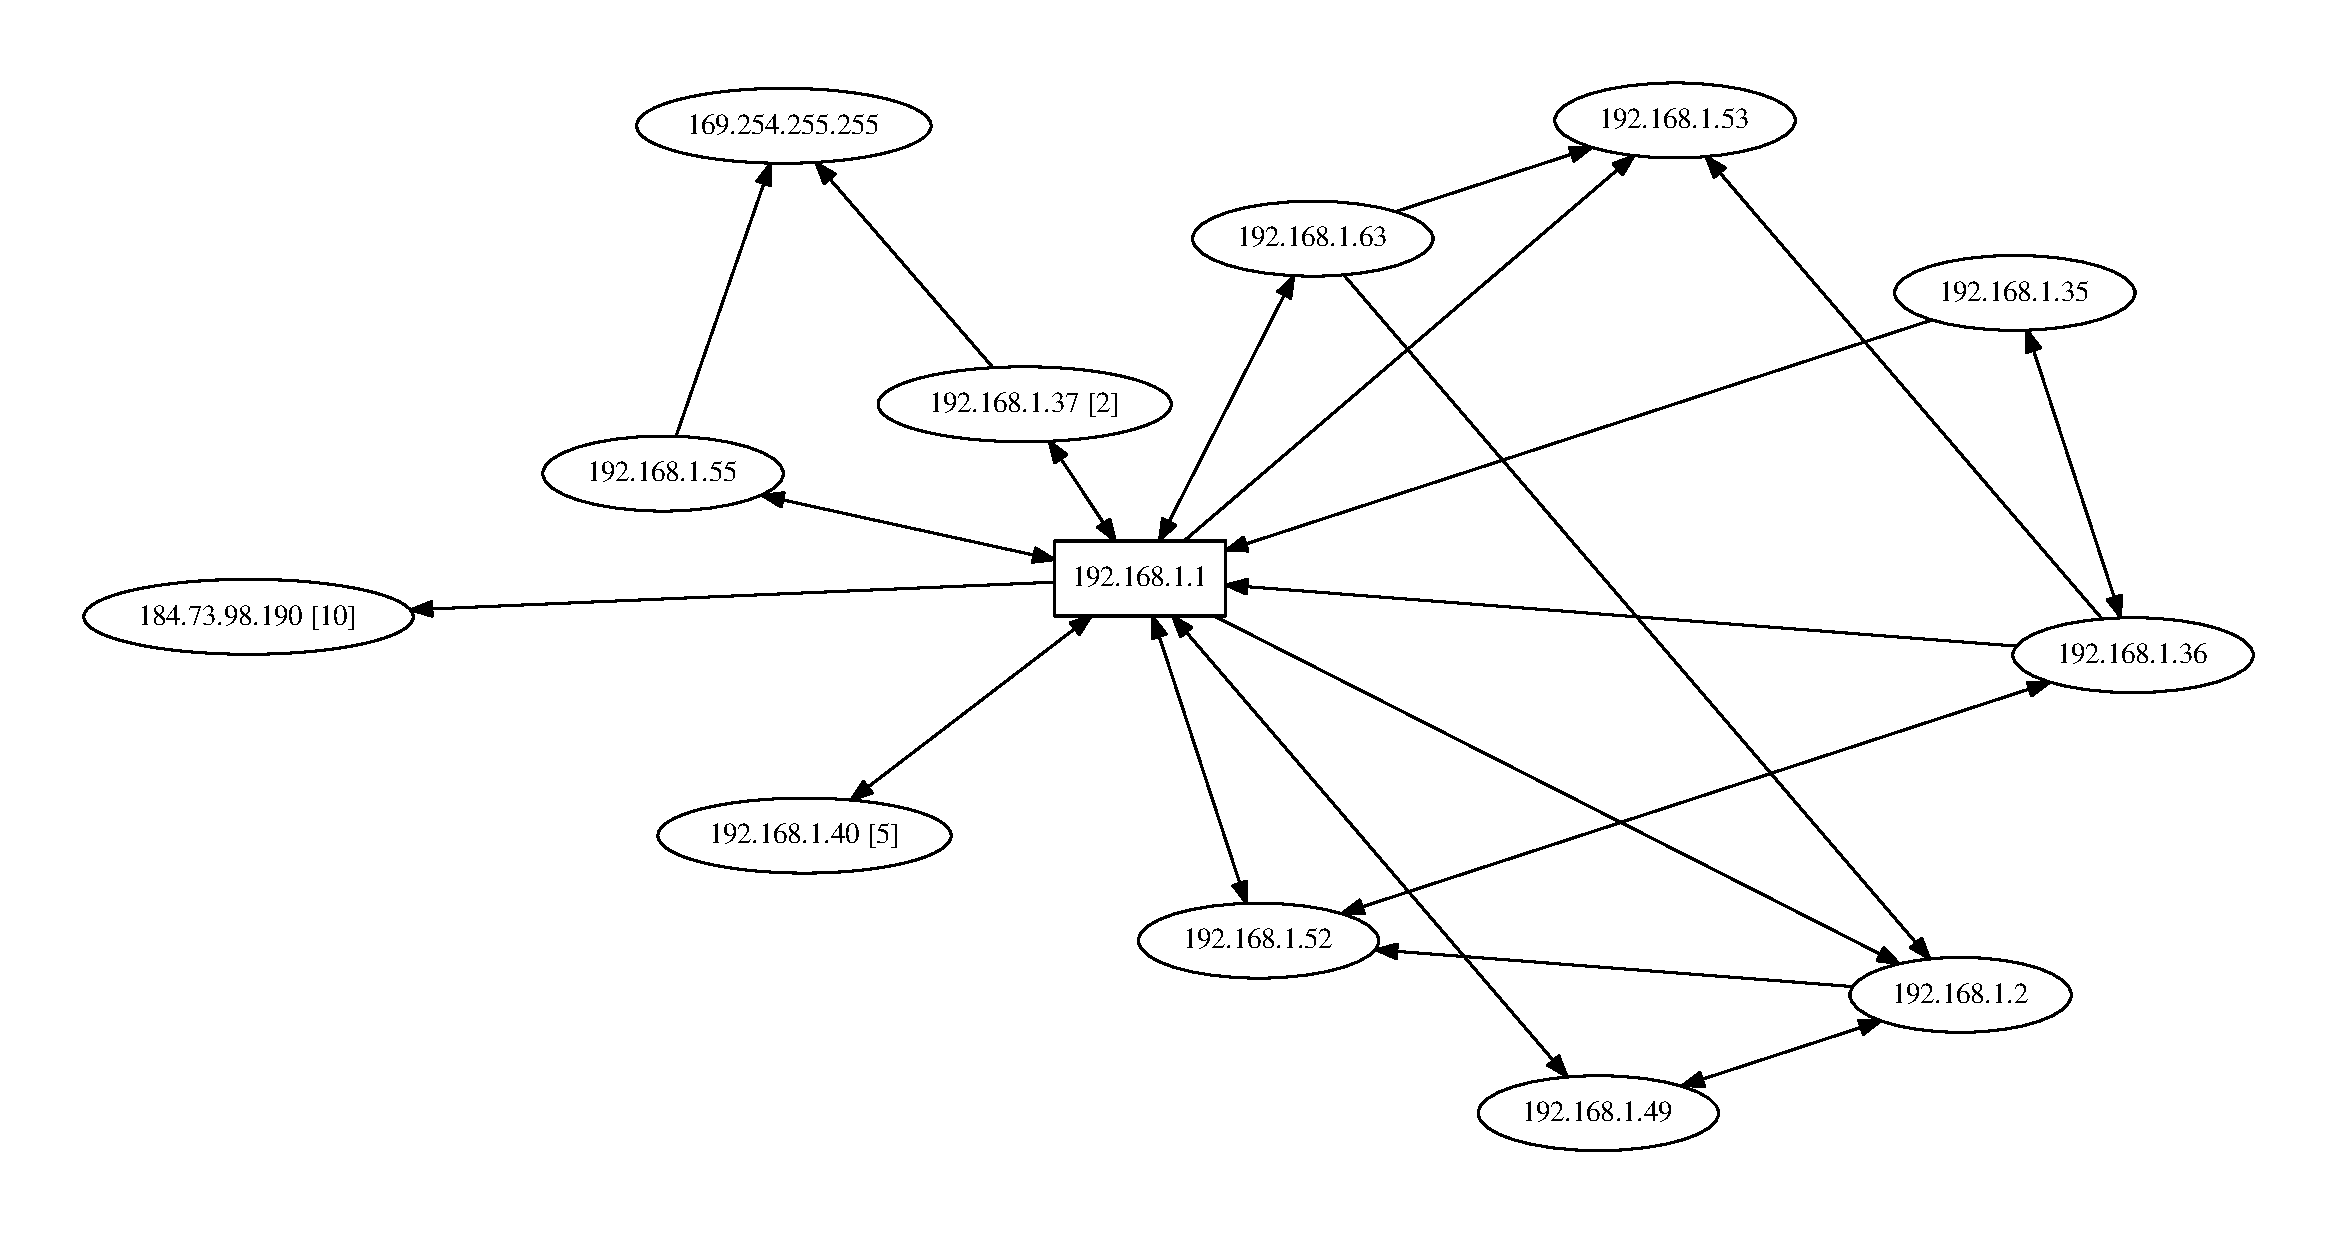
\includegraphics[width=8.5cm]{exp_empresa/grafico2.pdf}
  \caption{  \normalfont Grafo de conectividad de la red, inferido de los paquetes who-has. Para ver con mayor detalle, se puede hacer zoom-in en el pdf. }
\end{figure}

Esperaremos que a partir de la fuente S1 se destaque algún dispositivo que corresponderá al default gateway configurado en la tabla de routeo de los host (el router de la red).

\begin{figure}[H]
  \centering
  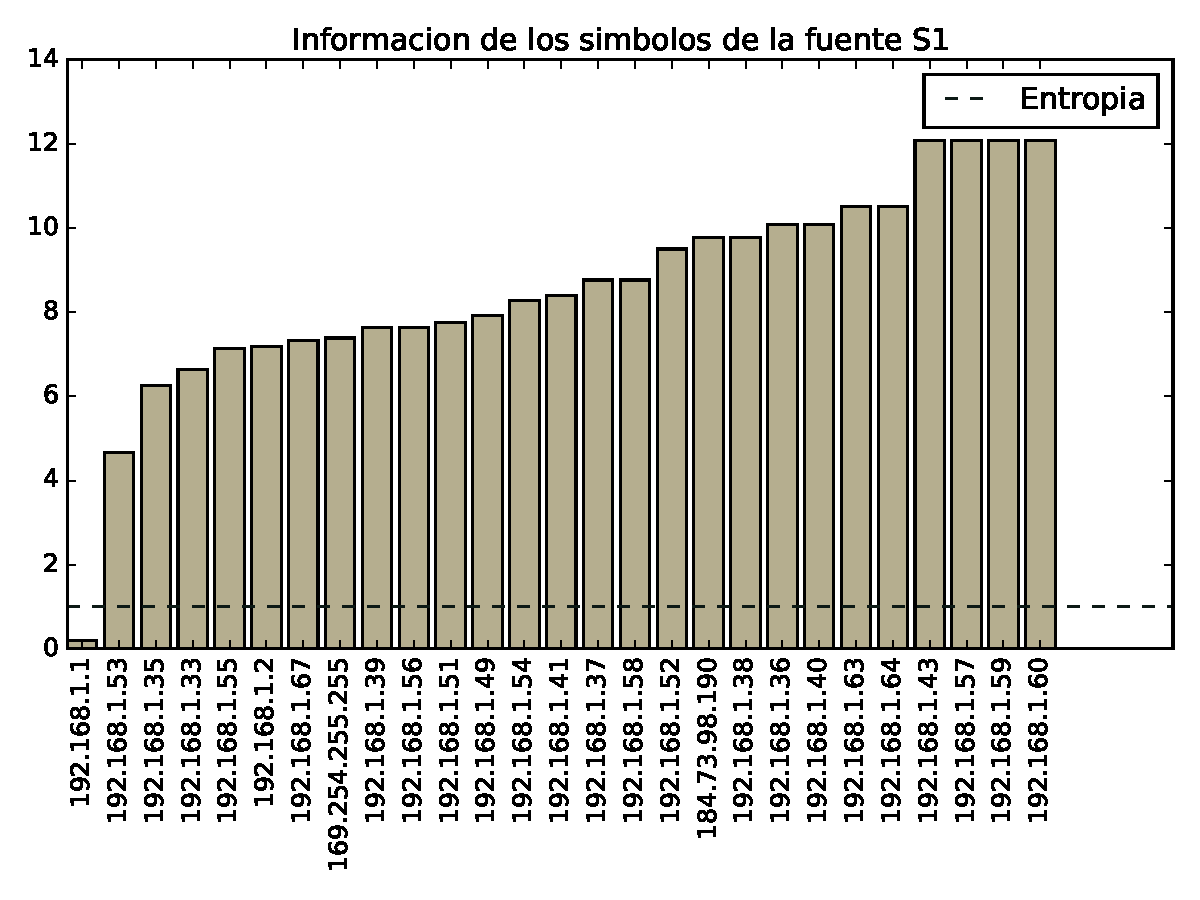
\includegraphics[width=8.5cm]{exp_empresa/grafico3.pdf}
  \caption{ \normalfont Información de los símbolos de la fuente S1: solamente los nodos con menor información son representados.}
\end{figure}

\subsection{Discusión}

Analicemos los resultados que vimos en la sección anterior.

En el gráfico correspondiente a la información de cada símbolo de la primera fuente, se puede observar, como predecíamos, que la información de los mensajes tipo broadcast es mayor. Sin embargo, a diferencia de la red wifi analizada en el primer experimento, la diferencia en este caso en menor debido a que la duración de la escucha en este experimento fue menor.

Como se ve en el gráfico, la entropía de la fuente está muy cercana a la entropía máximo debido a que la diferencia entre la información aportada por cada símbolo no es tan alta.

En el gráfico de topología de la red se puede observar al menos 15 direcciones de IP correspondientes a una misma red: 192.168.1.0 con una máscara de red 255.255.255.0 ya que todos los dispositivos tienen como último octeto valores entre 1 y 254. 

El dispositivo distinguido tiene como IP 192.168.1.1, que es la dirección usada normalmente para el router de la red, que se corresponde con el default/gateway configurado en los hosts.

En el grafo de la red se puede ver claramente como todos los dispositivos de la red local se comunican con el que consideramos es el router, para acceder quizás a algún servidor externo, representado en el nodo con la IP 184.73.98.190. Notar que este nodo tiene un [10] debido a que hay 10 nodos con las mismas aristas, es decir que aparecen como destino de algún paquete enviado por el router, y no pertenecen a la red local.

Además, se puede notar que los hosts de la red local se comunican entre sí, fenómeno que no se observa en la red de Starbucks. Esto se debe a que en una red de tipo empresarial, los dispositivos locales tienden a comunicarse entre sí, por lo que se envían paquetes ARP preguntando por las ips de los otros hosts de la red.

Por último, se puede observar la aparición del nodo 169.254.255.255, que como se mencionó anteriormente, corresponde a una dirección por default que se asignan los dispositivos debido a que DHCP no funcionó correctamente al asignar la ip.



